
\documentclass[12pt]{article}

\usepackage[utf8]{inputenc}
\usepackage[greek, english]{babel}

% Packages
\usepackage{alphabeta}
\usepackage{amsmath}
\usepackage{amsthm}
\usepackage{caption}
\usepackage{color}
\usepackage{float}
\usepackage{fullpage}
\usepackage{graphicx}
\usepackage{hyperref}
\usepackage{latexsym}
\usepackage{listings}
\usepackage{pxfonts}
\usepackage{stackrel}
\usepackage{subfig}
\usepackage{tikz}
\usepackage{titlesec}

% Commands
\newcommand{\N}{\mathbb{N}}
\newcommand{\R}{\mathbb{R}}
\newcommand{\abs}[1]{\left\lvert#1\right\rvert}
\newcommand{\code}[2]{\lstinputlisting[caption={#2}]{#1}}
\newcommand{\margin}{\hspace{4pt}}
\newcommand{\norm}[1]{\left\lVert#1\right\rVert}

% Environments
\newenvironment{matlab}
	{\begin{figure}[H]\centering\captionsetup{justification=centering}}
	{\end{figure}}

\newenvironment{rcases}
	{\left.\begin{aligned}}
	{\end{aligned}\right\rbrace}

% Python Syntax Highlighting
\definecolor{string_color}{RGB}{0, 161, 13}
\definecolor{comment_color}{RGB}{46, 46, 46}
\definecolor{keyword_color}{RGB}{0, 112, 191}
\definecolor{background_color}{RGB}{250, 250, 250}

\lstset{
    framesep=15pt,
    xleftmargin=15pt,
    xrightmargin=15pt,
    language=Python,
    captionpos=b,
    numbers=right,
    numberstyle=\small\ttfamily,
    frame=lines,
    showspaces=false,
    showtabs=false,
    breaklines=true,
    showstringspaces=false,
    breakatwhitespace=true,
    commentstyle=\color{comment_color}\textit,
    keywordstyle=\bfseries\color{keyword_color}\textbf,
    stringstyle=\color{string_color}\textit,
    morekeywords={self, lambda, __init__, __del__, __name__, for, in, not, and, or, :},
    basicstyle=\small\ttfamily,
    tabsize=4,
    keepspaces=true,
    columns=flexible,
    backgroundcolor=\color{background_color}
}

% Links
\hypersetup{
    colorlinks=true,
    linkcolor=blue,
    filecolor=magenta,
    urlcolor=cyan,
}

% Lengths
\setlength{\parindent}{0in}
\setlength{\oddsidemargin}{0in}
\setlength{\textwidth}{6.5in}
\setlength{\textheight}{10in}
\setlength{\topmargin}{-1.0in}
\setlength{\headheight}{18pt}

\titlespacing*{\subsection}
{0pt}{5.5ex plus 1ex minus .2ex}{4.3ex plus .2ex}

\title{\hugeΥπολογιστική Γεωμετρία\\Τρίτη Εργασία}
\author{Σιώρος Βασίλειος - 1115201500144\\Ανδρινοπούλου Χριστίνα - 1115201500006}
\date{Ιούνιος 2020}

\begin{document}

\maketitle

\pagenumbering{gobble}

\pagebreak


\subsection*{1. Compute Voronoi diagrams of different sets of vertices of your choice using
    the routine \textit{Voronoi} (and its companion \textit{voronoi\_plot\_2d} for visualization) from the module
    \textbf{scipy.spatial}. Plot your results.}

\begin{matlab}
    \includegraphics{images/voronoi/10_0.png}
    \caption{The Voronoi diagram of 10 random points with a random seed of 0}
\end{matlab}

\begin{matlab}
    \includegraphics{images/voronoi/10_10.png}
    \caption{The Voronoi diagram of 10 random points with a random seed of 10}
\end{matlab}

\begin{matlab}
    \includegraphics{images/voronoi/20_0.png}
    \caption{The Voronoi diagram of 20 random points with a random seed of 0}
\end{matlab}

\begin{matlab}
    \includegraphics{images/voronoi/20_10.png}
    \caption{The Voronoi diagram of 20 random points with a random seed of 10}
\end{matlab}

\begin{matlab}
    \includegraphics[scale=0.140]{images/help/voronoi.png}
    \caption{How to run the code}
\end{matlab}

\pagebreak

\subsection*{2. Using the routine \textit{Delaunay} in the module \textbf{scipy.spatial} compute the Delaunay
    triangulation of different sets of vertices of your choice and plot your results.}

\begin{matlab}
    \includegraphics{images/delaunay/10_0.png}
    \caption{The Delaunay triangulation of 10 random points with a random seed of 0}
\end{matlab}

\begin{matlab}
    \includegraphics{images/delaunay/10_10.png}
    \caption{The Delaunay triangulation of 10 random points with a random seed of 10}
\end{matlab}

\begin{matlab}
    \includegraphics{images/delaunay/20_0.png}
    \caption{The Delaunay triangulation of 20 random points with a random seed of 0}
\end{matlab}

\begin{matlab}
    \includegraphics{images/delaunay/20_10.png}
    \caption{The Delaunay triangulation of 20 random points with a random seed of 10}
\end{matlab}

\begin{matlab}
    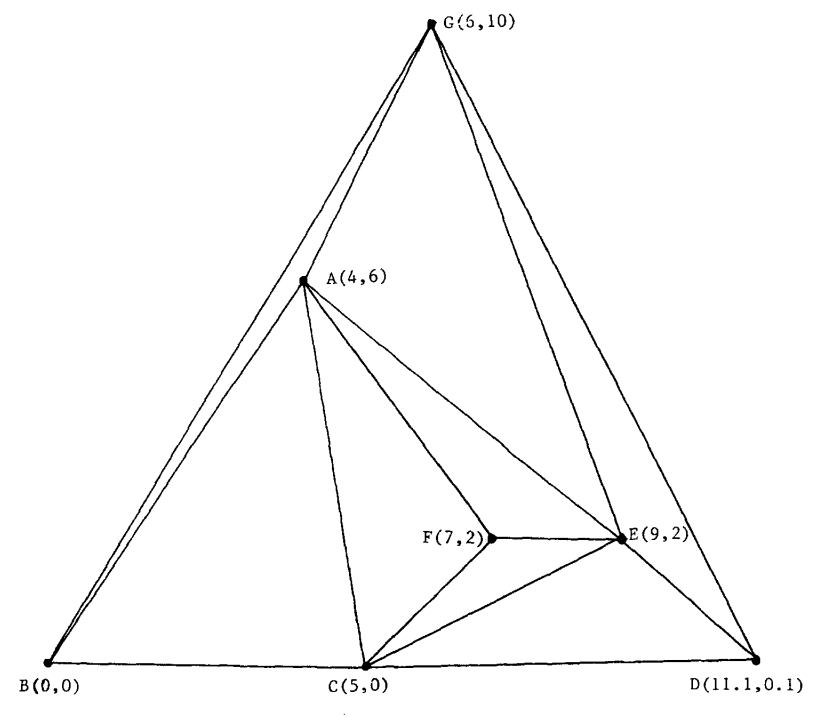
\includegraphics[scale=0.140]{images/help/delaunay.png}
    \caption{How to run the code}
\end{matlab}

\pagebreak

\subsection*{3. Compute the shortest path of different set of vertices of your choice in a tri-angulation. By a path in this setting, we mean a chain of edges of this triangulation. Use the
    methods in the package \textbf{scipy.sparse.csgraph}.}

\begin{matlab}
    \includegraphics{images/shortest_path/10_0.png}
    \caption{One of the shortest paths in a triangulation of 10 random points with a random seed of 0}
\end{matlab}

\begin{matlab}
    \includegraphics{images/shortest_path/10_10.png}
    \caption{One of the shortest paths in a triangulation of 10 random points with a random seed of 10}
\end{matlab}

\begin{matlab}
    \includegraphics{images/shortest_path/20_0.png}
    \caption{One of the shortest paths in a triangulation of 20 random points with a random seed of 0}
\end{matlab}

\begin{matlab}
    \includegraphics{images/shortest_path/20_10.png}
    \caption{One of the shortest paths in a triangulation of 20 random points with a random seed of 10}
\end{matlab}

\begin{matlab}
    \includegraphics[scale=0.140]{images/help/shortest_path.png}
    \caption{How to run the code}
\end{matlab}

\pagebreak

\subsection*{4. Experiment yourself with the \textit{.encloses\_point} and \textit{.encloses} methods of the
    \textbf{sympy.geometry} module using polygons or circles to check if they contain certain points of
    your choice. Do the same with \textit{contains\_point} or \textit{contains} points from the Path class from the
    libraries of \textbf{matplotlib.path}.}

\begin{matlab}
    \includegraphics{images/encloses_contains/encloses.png}
    \caption{Using the \textit{encloses} method}
\end{matlab}

\begin{matlab}
    \includegraphics{images/encloses_contains/encloses_point.png}
    \caption{Using the \textit{encloses\_point} method}
\end{matlab}

\begin{matlab}
    \includegraphics{images/encloses_contains/diff.png}
    \caption{Comprtin the \textit{encloses} and \textit{contains} methods}
\end{matlab}

\begin{matlab}
    \includegraphics[scale=0.140]{images/help/encloses_contains.png}
    \caption{How to run the code}
\end{matlab}

\pagebreak

\subsection*{5. The problem of finding the Voronoi cell that contains a given location is
    equivalent to the search for the nearest neighbor. We can always perform this search with a
    brute force algorithm, but in general there are more elegant and less complex approaches to
    this problem like the kd-trees. In the \textbf{scipy} use the class \textit{KDTree} to perform some experiments
    of your choice.}

Δεδομένου ενός συνόλου σημείων ορίζεται το αντίστοιχο Voronoi διάγραμμα. \\

Θα επιχειρήσουμε να υπολογίσουμε τα Voronoi διαγράμματα διάφορων συνόλων σημείων στον δισδιάστατο χώρο,
με τη βοήθεια του αλγορίθμου K κοντινότερων γειτόνων. \\

Δεδομένου ενός συνόλου εκπαίδευσης \( P \), του οποίου το Voronoi διάγραμμα επιθυμούμε
να υπολογίσουμε, ορίζουμε το meshgrid το οποίο ορίζεται από τα σημεία \\

\[ (\min_{\forall p \in P} p.x), \min_{\forall p \in P} p.y)) \]

\[ (\max_{\forall p \in P} p.x), \max_{\forall p \in P} p.y)) \]

Αφού εκπαιδεύσουμε το μοντέλο μας, κατηγοριοποιούμε κάθε σημείο που ανήκει
στο meshgrid, έτσι ώστε να προκύψει το Voronoi διάγραμμα. \\

\begin{matlab}
    \includegraphics{images/kdtree/force/1_01_02250998.png}
    \caption{Using brute force in order to find the single closest neighbor of 80 points}
\end{matlab}

\begin{matlab}
    \includegraphics{images/kdtree/tree/1_01_04772699.png}
    \caption{Using KD-Tree neighborhood look-up in order to find the single closest neighbor of 80 points}
\end{matlab}

\begin{matlab}
    \includegraphics{images/kdtree/force/3_005_10156662.png}
    \caption{Using brute force in order to find the 3 closest neighbors of 160 points}
\end{matlab}

\begin{matlab}
    \includegraphics{images/kdtree/tree/3_005_21572421.png}
    \caption{Using KD-Tree neighborhood look-up in order to find the 3 closest neighbors of 160 points}
\end{matlab}

\begin{matlab}
    \includegraphics{images/kdtree/force/5_0005_1032422123.png}
    \caption{Using brute force in order to find the 5 closest neighbors of 1600 points}
\end{matlab}

\begin{matlab}
    \includegraphics{images/kdtree/tree/5_0005_2527861562.png}
    \caption{Using KD-Tree neighborhood look-up in order to find the 5 closest neighbors of 1600 points}
\end{matlab}

\pagebreak

Παρ' ότι η μέθοδος των KD-Δέντρων είναι προσεγγιστική και δεν εγγυάται
ότι θα βρεί τους Κ πραγματικά κοντινότερους γείτονες,
στην προκείμενη περίπτωση η απόκλιση του τελικού αποτελέσματος
σε σχέση με τη μέθοδο ωμής βίας είναι ουσιαστικά ανύπαρκτη. \\

Ωστόσο, αυτό που είναι σίγουρο είναι πώς η μέθοδος των KD-Δέντρων είναι σημαντικά γρηγορότερη,
όπως φαίνεται και από τα παρακάτω δεδομένα. \\

\begin{center}
    \begin{tabular}{ |c|c|c|c|c| }
        \hline\hline
        Type  & Neighbors & Predictions & Time        & Efficiency         \\
        \hline\hline
        force & 1         & 800         & 43271.45770 & 1                  \\
        \hline
        force & 1         & 160         & 2870.635500 & 1                  \\
        \hline
        force & 1         & 80          & 477.2699000 & 1                  \\
        \hline
        force & 3         & 800         & 54532.69620 & 1                  \\
        \hline
        force & 3         & 160         & 2157.242100 & 1                  \\
        \hline
        force & 3         & 80          & 546.4535000 & 1                  \\
        \hline
        force & 5         & 1600        & 252786.1562 & 1                  \\
        \hline
        force & 5         & 800         & 63132.58790 & 1                  \\
        \hline
        tree  & 1         & 800         & 20512.63240 & 2.1095029080714185 \\
        \hline
        tree  & 1         & 160         & 899.3549000 & 3.1918828707109950 \\
        \hline
        tree  & 1         & 80          & 225.0998000 & 2.1202591028512687 \\
        \hline
        tree  & 3         & 800         & 21523.35190 & 2.5336525859617620 \\
        \hline
        tree  & 3         & 160         & 1015.666200 & 2.1239675988036226 \\
        \hline
        tree  & 3         & 80          & 211.0624000 & 2.5890613392058460 \\
        \hline
        tree  & 5         & 1600        & 103242.2123 & 2.4484767477226947 \\
        \hline
        tree  & 5         & 800         & 21571.52390 & 2.9266633267388213 \\
        \hline
    \end{tabular}
\end{center}

\begin{matlab}
    \includegraphics[scale=0.140]{images/help/kdtree.png}
    \caption{How to run the code}
\end{matlab}

\pagebreak

\end{document}
